\section*{Оценка количества атомов}


\textbf{Связь с количеством атомов}. 
Если атом движется на скорости $v$, то доплеровское смещение приведет к резонансу на частоте
\begin{equation*}
	\nu(v) = \nu_0 \left(1 + \frac{v}{c}\right),
	\hspace{0.5cm} \Rightarrow \hspace{0.5cm}
	d \nu = \frac{\nu_0}{c} \d v.
\end{equation*}
где $\nu_0$ -- резонансная частота.
Мощность детектируемого излучения $J(\nu) \d \nu$ связана с плотностью атомов $n(v) \d v$. 
% через коэффициент $\kappa$:
% \begin{equation*}
% 	J(\nu) = \kappa \cdot n(v),
% 	\hspace{0.5cm} \Rightarrow \hspace{0.5cm}
% 	J(\nu) \d \nu = \kappa n(v) \nu_0 \frac{dv}{c}.
% \end{equation*}
Связь интеграла по мощности излучения $\mathcal I = \int J(\nu) \d \nu$ с количеством атомов $N = \int n(v) \d v$ запишем в виде
\begin{equation*}
	\mathcal I = \kappa N.
\end{equation*}
% \begin{equation*}
% 	\mathcal I = \frac{\kappa \nu_0}{c} N.
% \end{equation*}

\textbf{Интегральная мощность излучения}. По расстоянию между пиками сверхтонкой структуры для ${}^6$Li (228 МГц) отмасштабируем развёртку. Из калибровки ФЭУ знаем, что мощности излучения в 1 нВт, соответсвует $4.7$~В, теперь можем найти $\mathcal I$, см. рис. \ref{fig:1}.

\begin{figure}[h]
    \centering
    \vspace{-4mm}
    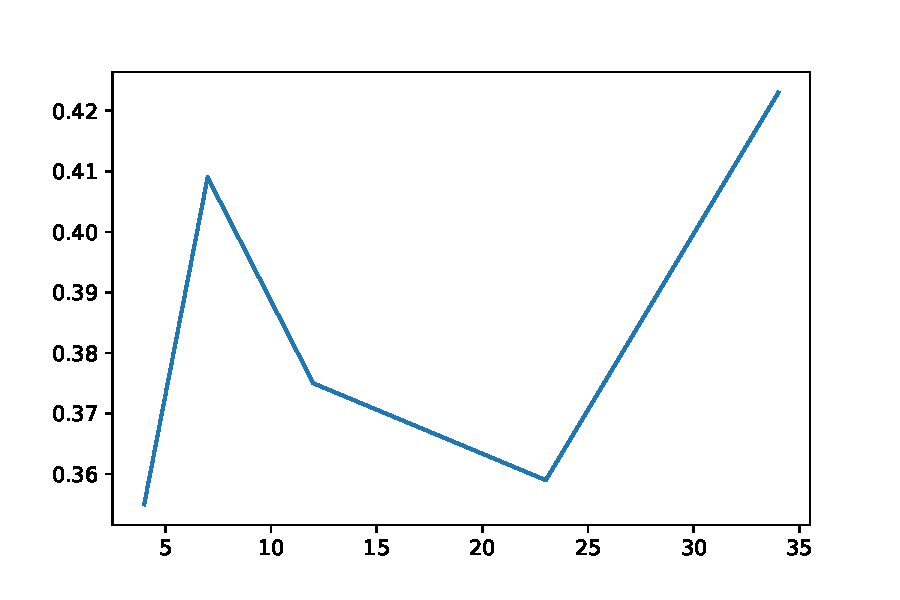
\includegraphics[width=0.4\textwidth]{D:/workspace/python/count_atoms/1.pdf}
    \hspace{5 mm} 
    \includegraphics[width=0.4\textwidth]{D:/workspace/python/count_atoms/3.pdf}
    \vspace{-4mm}
    \caption{Численная оценка параметров пиков}
    \label{fig:1}
\end{figure}
\vspace{-4mm}


Считая пики гауссовыми, можем оценить их параметры (приведены в единицах в соответсвие с графиком):
\begin{align*}
	G(\nu) = A \exp\left(- \frac{(\nu-\nu_c)^2}{2 \sigma^2}\right),
	\hspace{10 mm} 
	&A_L = 0.0362,
	\hspace{2.5 mm} 
	\nu_R = 601, 
	\hspace{2.5 mm} 
	\sigma_L = 48.2, \\
	&A_R = 0.0121,
	\hspace{2.5 mm} 
	\nu_L = 829,
	\hspace{2.5 mm} 
	\sigma_R = 64.3.
\end{align*}
Тогда находим $\mathcal I$ для левого пика
\begin{equation*}
	\mathcal{I} = A_L \sqrt{2 \pi} \sigma_L \approx 4.4 \ \text{нВт}\cdot\text{МГц}.
\end{equation*}
На самом деле корректнее будет учесть, что уширение лазера $\sim 1$ МГц \red{(но это не точно)}, поэтому измерялись не нВт, а нВт/МГц, а значит с размрностью всё впорядке
\begin{equation*}
	\mathcal{I} \approx 4.4\ \text{нВт}. 
\end{equation*}


\textbf{Телесный угол}. Спонтанное излчение происходит в $4 \pi$, дектируем только некоторый телесный угол $\Omega$. 
Расстояние $L$ от флюорисцирующих атомов до линзы равно $\approx 90$ мм, диаметр линзы $D$ равен $52$ мм.

Телесный угол, выделяемый конусом с углом раствора $\alpha$, высоты $L$ и радиуса $D/2$, может быть найден, как
\begin{equation*}
	\Omega = 2 \pi \left(1 - \cos \frac{\alpha}{2}\right) = 2 \pi \left(1 - \frac{L}{\sqrt{L^2 + D^2/4}}\right) \approx	2 \pi \cdot 0.039.
\end{equation*}
откуда знаем связь детектируемого излучения $J$ с полным излучением $J_0(\nu)$:
\begin{equation*}
	J_0 (\nu) = \frac{4 \pi}{\Omega} J(\nu).
\end{equation*}

\textbf{Интенсивность излучения}. Интенсивность излучения фотона можем найти в виде
\begin{equation*}
	\mathcal J  = \frac{4}{3 c^3} \omega^4 d^2 = \frac{\hbar \omega}{\tau}.
\end{equation*}
Вообще, зная время жизни уровня ${}^6$Li, можем оценить $\mathcal J$ с $\tau = 27.2$ нс.

Интенсивность излучения лазера много больше интенсивности насыщения ${}^6$Li (\red{проверить}), поэтому можем считать, что половина атомов поддерживается в возбужденном состоянии, тогда
\begin{equation*}
	\mathcal{J} \frac{\d N}{2} \approx \frac{1}{2} \frac{\hbar \omega}{\tau} n(v) \d v = J_0(\nu) \d \nu = \frac{4 \pi}{\Omega} J(\nu) \d \nu,
\end{equation*}
откуда находим искомую связь
\begin{equation*}
	\kappa = \frac{J(\nu) \d \nu}{ n(v) \d v} = \frac{1}{2} \frac{\Omega}{4\pi}  \frac{\hbar \omega}{\tau}.
\end{equation*}


\textbf{Количество атомов}. Собирая всё вместе, находим
\begin{equation*}
	N = \left(\frac{1}{2} \frac{\Omega}{4\pi} \frac{\hbar \omega}{\tau}\right)^{-1} \mathcal{I} \approx	 4 \cdot 10^{4}.
\end{equation*}

\textbf{Количество атомов в секунду}. Знаем, что атомы движутся на скорости $v_0 \approx 1$ км/c \red{(написать точнее)}. 
Лазерный пучок выделяет область шириной $w \sim 3$ мм, тогда можем найти количество атомов $\mathcal N$, которое вылетает из печки за одну секунду
\begin{equation*}
	t \sim \frac{w}{v_0} \sim 3\ \mu\text{с},
	\hspace{0.5cm} \Rightarrow \hspace{0.5cm}
	\mathcal N = \frac{N}{t} \approx 10^{10}\ \frac{\text{атом}}{\text{c}}.
\end{equation*}